\chapter{Introdução}

%As citações são feitas usando o comando~\texttt{\textbackslash cite}. Para usar colchetes nas citações, use o comando \texttt{\textbackslash citeC}. Exemplo


\section{Contextualização e Definição do Problema}

\section{Introdução à Conceituação do Efeito  de modulação\textit{Reverb}}
	\subsection{Aplicabilidade}
		Numa sala, ou em qualquer ambiente acústico, existe um caminho direto pelo qual uma fonte de áudio qualquer pode ser ouvida, no entanto, as respectivas ondas sonoras também podem fluir em caminhos mais longos devido a, por exemplo, reflexão das paredes, do teto, de objetos, antes delas chegarem ao receptor.
		
		A energia envolvida som dessas reflexões, as quais viajam essas distâncias maiores do que o som emitido no caminho direto, são parcialmente absorvidas pelas superfícies, logo elas chegam ao receptor com um som mais "fraco" que o som direto.
		
		Essas amostras de som atrasadas e atenuadas ocorridas no evento da emissão do som original é o que denominamos de \textit{reverbaração}.
		
		Muito embora possa parecer algo sim, o efeito de reverberação é muito mais que uma série de ecos. 

\section{Comparativo entre soluções de Hardware}

		No mercado, atualmente, poucas são as empresas possuem em seu portfólio esse tipo de efeito modulante com essa característica. Vale destacar que o efeito puramente de reverberação já é notoriamente conhecido e manipulado por diversos hardwares e softwares no mercado. Note-se que estamos falando do efeito adicional incorporado ao produto que é o chamado \textit{shimmer}.
		
		

	\subsection{Micontroladores e DSP's}

		O termo sistemas embarcados constituem circuitos eletrônicos que utilizam processadores digitais (microprocessadores ou microcontroladores, etc.) em aplicações dedicadas para determinado equipamento ou produtos.
		
		Os microcontroladores, diferentemente dos microprocessadores, em geral, possuem todos os periféricos necessários num único chip. Seu tamanho também é muito pequeno, mesmo contendo vários periféricos como: memórias, barramentos, \textit{timers}, portas de comunição, conversores de sinal analógicos para digital etc.
		
		Por outro lado, esses dispositivos possuem um desempenho menor que os microprocessadores, mas são ideais em aplicações que necessitam de menores dimensões, tempo e custos.
		
		As linguagens de programação das unidades processadores de sistemas embarcados podem variar, mas em geral, se limitam às linguagens C/C++, \textit{Assembly} e \textit{Java}.
		
		Nessa linha, temos ainda o processador digital de sinais (DSP - \textit{Digital Signal Processing}) e pode definir tanto o processador quanto o processo em si. Esse tipo de tratamento exige um alto desempenho para aplicações numéricas em tempo real.
		
		Os DSP's são construídos para computar de forma eficiente equações de diferenças e algoritmos de transformadas diversas (como a \textit{Fast Fourier Transform} - FFT). As aplicações dos DSP's, em suma, estão relacionadas com sistemas de controle de alta velcodiade, realizações de filtros digitais, transformadas rápidas de \textit{Fourier}, processamento de sons e imagens, entre outras.

	\subsection{Hardwares Comerciais do Efeito \textit{Reverb - Shimmer}}
	
	\subsection{Microcontrolador MSP430F5529 e TMS320}
	
	Foram utilizados ao longo do projeto como soluções de hardware essencialmente o \textit{microntrolador launchpad MSP430F5529}.
	
	Não obstante foram apontados na subseção anterior a respeito das limitações do hardware para tratamento de sinais de áudio em tempo real, o escopo do trabalho levou em consideração a economicidade do hardware em questão, bem como a utilização de operações no domínio do tempo, sem utilização de etapas intermediárias como realização da transformada de \textit{Fourier} para manipulação do sinal de áudio. %melhorar esse texto
	
	Além disso, o projeto teve uma participação do desempenho do TSM320 C2000 o qual, devido ao tempo de aprendizagem do DSP para correta aplicabilidade no projeto, não fora possível. %melhorar o texto


\section{Diagrama de Bloco do Projeto}

	Nesta parte do trabalho, é mostrado de maneira abstrata os blocos necessários para que obtenha a saída do sistema desejado, ou seja, o efeito do \textit{Reverb} com \textit{Shimmer} implementado em software e executado em hardware.
	
	Temos aqui na figura \ref{bloco-principal} um sinal analógico oriundo e um instrumento musical - guitarra, que passa por um processador de som digital - DSP o qual faz toda o trabalho de tratamento do sinal analógico convertido para amostras digitais. Aplicando, portanto, nesse contexto, um filtro de resposta finita; um algoritmo de seleção de frequências denominado \textit{pitch-shifter} e por fim realimentando o sistema acrescentando um pequeno atraso temporal (\textit{delay}).
	
	\begin{figure}[!h t b]
		\label{bloco-principal}
		\centering
		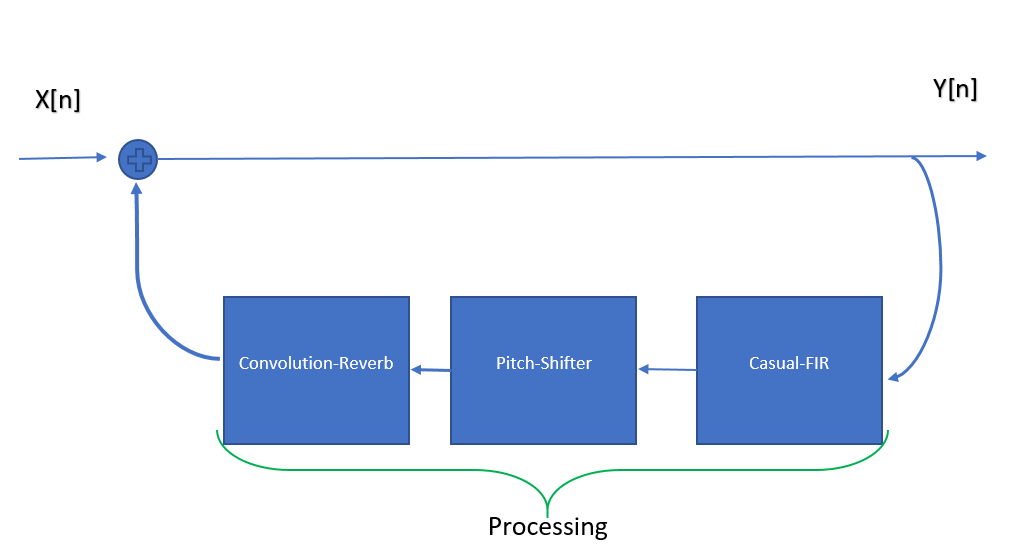
\includegraphics[scale=0.5]{./figuras/diagrama_bloco_principal.PNG}
		\caption{Diagrama de Blocos Principal do Projeto.}
	\end{figure}

	Como uma lei de controle de malha fechada podemos ilustrar (figura \ref{signal_principal}) também como um diagrama de fluxo de sinais da seguinte forma:
	
	\begin{figure}[!h t b]
		\label{signal_principal}
		\centering
		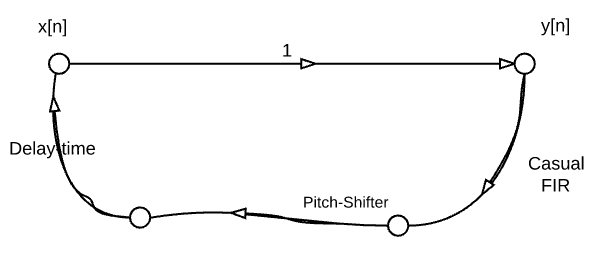
\includegraphics[scale=0.5]{./figuras/fluxo_de_sinais_principal.png}
		\caption{Diagrama de Fluxo de Sinais do Projeto.}	
	\end{figure}
	
	
	
	
	
	

